\documentclass[12pt, letterpaper]{article}
\usepackage{graphicx}
\usepackage[margin=1in]{geometry}
\usepackage{amsmath, amssymb, amsthm, mathrsfs}
\usepackage{fancyhdr}
\usepackage{tikz}
\usepackage{enumerate}
\usepackage{cancel}
\usetikzlibrary{positioning}
\usepackage[utf8]{inputenc}
\usepackage{xcolor}

\title{HW 1.1}
\author{Your Name}
\date{\today}

\pagestyle{fancy}
\renewcommand{\headrulewidth}{0pt}
\renewcommand{\footrulewidth}{0pt}
\fancyhf{}
\rhead{
    Zack Abdirashid\\
    1/20/26 \\
    MATH 405
}
\rfoot{Page \thepage}

\begin{document}

\paragraph{\underline{1.1} \\ \\} 

\textbf{2. (a)} \textit{Suppose four teams, the Aces, the Birds, the Cats, and the Dogs, play each other once. The Aces beat all three opponents except the Birds. The Birds lose to all opponents except the Aces. The Dogs beat the Cats. Represent the results of these games with a directed graph.}

\begin{align*}
    \text{* A vertex $x$ pointing to a vertex $y$ implies $x$ beat $y$.}
\end{align*}

\begin{center}
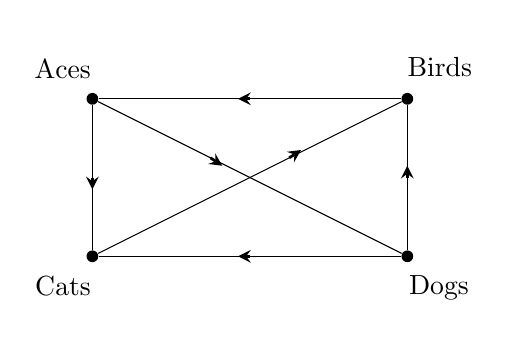
\begin{tikzpicture}[>=stealth, every node/.style={circle,fill,minimum size=3pt,inner sep=1.5pt}]
    \node[label=above left:Aces] (aces) at (0,2) {};
    \node[label=above right:Birds] (birds) at (4,2) {};
    \node[label=below left:Cats] (cats) at (0,0) {};
    \node[label=below right:Dogs] (dogs) at (4,0) {};
    
    % Aces to Cats (left edge, arrow pointing down)
    \draw (aces) -- (cats);
    \draw[->,line width=1pt] (0,1) -- (0,0.85);
    
    % Cats to Birds (bottom-left to top-right diagonal, arrow pointing towards Birds)
    \draw (cats) -- (birds);
    \draw[->,line width=1pt] (2.5,1.25) -- (2.65,1.35);
    
    % Dogs to Birds (right edge, arrow pointing up)
    \draw (dogs) -- (birds);
    \draw[->,line width=1pt] (4,1) -- (4,1.15);
    
    % Aces to Dogs (top-left to bottom-right diagonal, arrow pointing from Aces towards Dogs)
    \draw (aces) -- (dogs);
    \draw[->,line width=1pt] (1.5,1.25) -- (1.65,1.15);
    
    % Birds to Aces (top edge, arrow pointing left)
    \draw (birds) -- (aces);
    \draw[->,line width=1pt] (2,2) -- (1.85,2);
    
    % Dogs to Cats (bottom edge, arrow pointing left)
    \draw (dogs) -- (cats);
    \draw[->,line width=1pt] (2,0) -- (1.85,0);
\end{tikzpicture}
\end{center}

\vspace{1em}

\textbf{(b)} \textit{A dominance order is a listing of teams such that the $i$th team in the order beats the $(i+1)$ st team. Find all dominance orders for (a).}
\\ \\
The possible dominance orders are:
\begin{align*}
\boxed{
\begin{array}{l}
(1)\ \text{Aces - Dogs - Cats - Birds} \\
(2)\ \text{Birds - Aces - Dogs - Cats} \\
(3)\ \text{Cats - Birds - Aces - Dogs} \\
(4)\ \text{Dogs - Cats - Birds - Aces}
\end{array}
}
\end{align*}
\vspace{2em}


\textbf{7.} \textit{Find all possibles matchings, or explain why none exists for the following graphs.}

\textbf{(a)} 

\begin{center}
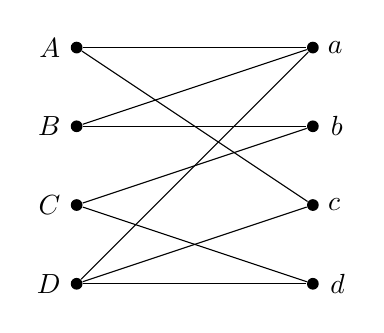
\begin{tikzpicture}[every node/.style={circle,fill,minimum size=1px,inner sep=1.5pt}]
    \node[label=180:$A$] (A) at (0,3) {};
    \node[label=180:$B$] (B) at (0,2) {};
    \node[label=180:$C$] (C) at (0,1) {};
    \node[label=180:$D$] (D) at (0,0) {};
    
    \node[label=0:$a$] (a) at (3,3) {};
    \node[label=0:$b$] (b) at (3,2) {};
    \node[label=0:$c$] (c) at (3,1) {};
    \node[label=0:$d$] (d) at (3,0) {};
    
    \draw (A) -- (a);
    \draw (A) -- (c);
    \draw (B) -- (a);
    \draw (B) -- (b);
    \draw (C) -- (b);
    \draw (C) -- (d);
    \draw (D) -- (a);
    \draw (D) -- (c);
    \draw (D) -- (d);
\end{tikzpicture}
\end{center}

\underline{Choose}: $(A, c)$

\begin{center}
\begin{tikzpicture}[every node/.style={circle,fill,minimum size=1px,inner sep=1.5pt}]
    \node[label=180:$B$] (B) at (0,2) {};
    \node[label=180:$C$] (C) at (0,1) {};
    \node[label=180:$D$] (D) at (0,0) {};
    
    \node[label=0:$a$] (a) at (3,2) {};
    \node[label=0:$b$] (b) at (3,1) {};
    \node[label=0:$d$] (d) at (3,0) {};
    
    \draw (B) -- (a);
    \draw (B) -- (b);
    \draw (C) -- (b);
    \draw (C) -- (d);
    \draw (D) -- (d);
    \draw (D) -- (a)
\end{tikzpicture}
\end{center}

\underline{Choose}: $(D, d)$

\begin{center}
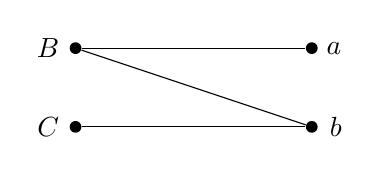
\begin{tikzpicture}[every node/.style={circle,fill,minimum size=1px,inner sep=1.5pt}]
    \node[label=180:$B$] (B) at (0,2) {};
    \node[label=180:$C$] (C) at (0,1) {};
    
    \node[label=0:$a$] (a) at (3,2) {};
    \node[label=0:$b$] (b) at (3,1) {};
    
    \draw (B) -- (a);
    \draw (B) -- (b);
    \draw (C) -- (b);
\end{tikzpicture}
\end{center}

\underline{Force}: $(C, b)$ (deg(C) = 1)
\begin{center}
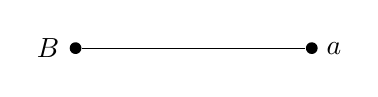
\begin{tikzpicture}[every node/.style={circle,fill,minimum size=1px,inner sep=1.5pt}]
    \node[label=180:$B$] (B) at (0,2) {};
    
    \node[label=0:$a$] (a) at (3,2) {};

    
    \draw (B) -- (a);
\end{tikzpicture}
\end{center}

\begin{align*}
    \Rightarrow 1) \ \boxed{\{(A, c), (C, b), (B, a), (D, d)\}}
\end{align*}

\underline{Backtrack} from (D,d)
\begin{center}
\begin{tikzpicture}[every node/.style={circle,fill,minimum size=1px,inner sep=1.5pt}]
    \node[label=180:$B$] (B) at (0,2) {};
    \node[label=180:$C$] (C) at (0,1) {};
    \node[label=180:$D$] (D) at (0,0) {};
    
    \node[label=0:$a$] (a) at (3,2) {};
    \node[label=0:$b$] (b) at (3,1) {};
    \node[label=0:$d$] (d) at (3,0) {};
    
    \draw (B) -- (a);
    \draw (B) -- (b);
    \draw (C) -- (b);
    \draw (C) -- (d);
    \draw (D) -- (a)
\end{tikzpicture}
\end{center}

\underline{Force}: (D,a), (C,d) (deg(D) = deg(d) = 1)
\begin{center}
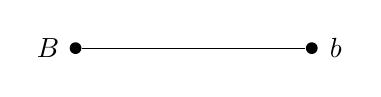
\begin{tikzpicture}[every node/.style={circle,fill,minimum size=1px,inner sep=1.5pt}]
    \node[label=180:$B$] (B) at (0,2) {};
    \node[label=0:$b$] (b) at (3,2) {};
    
    \draw (B) -- (b);
\end{tikzpicture}
\end{center}

\begin{align*}
    \Rightarrow \ 2) \ \boxed{(D, a), (C, d), (B, b), (A,c)}
\end{align*}

\underline{Backtrack} from (A, c)
\begin{center}
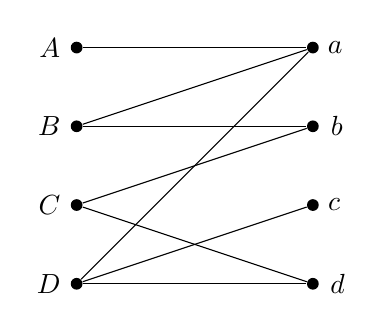
\begin{tikzpicture}[every node/.style={circle,fill,minimum size=1px,inner sep=1.5pt}]
    \node[label=180:$A$] (A) at (0,3) {};
    \node[label=180:$B$] (B) at (0,2) {};
    \node[label=180:$C$] (C) at (0,1) {};
    \node[label=180:$D$] (D) at (0,0) {};
    
    \node[label=0:$a$] (a) at (3,3) {};
    \node[label=0:$b$] (b) at (3,2) {};
    \node[label=0:$c$] (c) at (3,1) {};
    \node[label=0:$d$] (d) at (3,0) {};
    
    \draw (A) -- (a);
    \draw (B) -- (a);
    \draw (B) -- (b);
    \draw (C) -- (b);
    \draw (C) -- (d);
    \draw (D) -- (a);
    \draw (D) -- (c);
    \draw (D) -- (d);
\end{tikzpicture}
\end{center}

\underline{Force}: (A,a) (deg(A) = 1)
\begin{center}
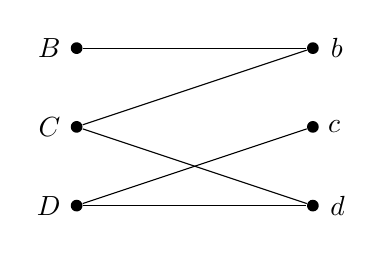
\begin{tikzpicture}[every node/.style={circle,fill,minimum size=1px,inner sep=1.5pt}]
    \node[label=180:$B$] (B) at (0,3) {};
    \node[label=180:$C$] (C) at (0,2) {};
    \node[label=180:$D$] (D) at (0,1) {};
    
    \node[label=0:$b$] (b) at (3,3) {};
    \node[label=0:$c$] (c) at (3,2) {};
    \node[label=0:$d$] (d) at (3,1) {};
    
    \draw (B) -- (b);
    \draw (C) -- (b);
    \draw (C) -- (d);
    \draw (D) -- (c);
    \draw (D) -- (d);
\end{tikzpicture}
\end{center}

\underline{Force}: (B,b) (deg(B) = 1)
\begin{center}
\begin{tikzpicture}[every node/.style={circle,fill,minimum size=1px,inner sep=1.5pt}]
    \node[label=180:$C$] (C) at (0,3) {};
    \node[label=180:$D$] (D) at (0,2) {};
    
    \node[label=0:$c$] (c) at (3,3) {};
    \node[label=0:$d$] (d) at (3,2) {};
    
    \draw (C) -- (d);
    \draw (D) -- (c)
\end{tikzpicture}
\end{center}

\begin{align*}
    \Rightarrow \ 3) \ \boxed{(A,a), (B,b), (D, c), (C,d)}    
\end{align*}

\begin{center}
    All choices have been exhausted, $\therefore$ all possible solutions have been found.    
\end{center}

\vspace{2em}

\textbf{(b)}

\begin{center}
\begin{tikzpicture}[every node/.style={circle,fill,minimum size=1px,inner sep=1.5pt}]
    \node[label=180:$A$] (A) at (0,3) {};
    \node[label=180:$B$] (B) at (0,2) {};
    \node[label=180:$C$] (C) at (0,1) {};
    \node[label=180:$D$] (D) at (0,0) {};
    
    \node[label=0:$a$] (a) at (3,3) {};
    \node[label=0:$b$] (b) at (3,2) {};
    \node[label=0:$c$] (c) at (3,1) {};
    \node[label=0:$d$] (d) at (3,0) {};
    
    \draw (A) -- (b);
    \draw (B) -- (a);
    \draw (B) -- (b);
    \draw (B) -- (c);
    \draw (B) -- (d)
    \draw (C) -- (b);
    \draw (D) -- (b);
    \draw (D) -- (d);
\end{tikzpicture}
\end{center}

\underline{Force}: $(B, a)$ ($\deg(a) = 1$)

\begin{center}
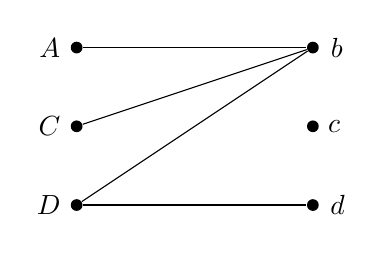
\begin{tikzpicture}[every node/.style={circle,fill,minimum size=1px,inner sep=1.5pt}]
    \node[label=180:$A$] (A) at (0,2) {};
    \node[label=180:$C$] (C) at (0,1) {};
    \node[label=180:$D$] (D) at (0,0) {};
    
    \node[label=0:$b$] (b) at (3,2) {};
    \node[label=0:$c$] (c) at (3,1) {};
    \node[label=0:$d$] (d) at (3,0) {};
    
    \draw (A) -- (b);
    \draw (C) -- (b);
    \draw (D) -- (b);
    \draw (D) -- (d);
\end{tikzpicture} 
\\
 $\Rightarrow$ No matching exists (either $A$ or $C$ will end up with degree 0 and $\deg(c) = 0$)
\end{center}



\vspace{1em}

\underline{Backtrack} from (B, a)

\begin{center}
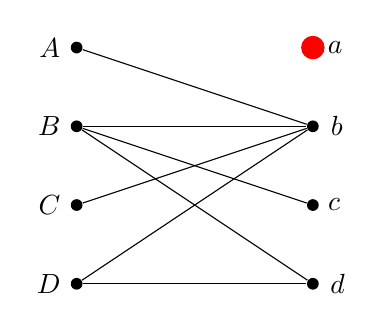
\begin{tikzpicture}[every node/.style={circle,fill,minimum size=1px,inner sep=1.5pt}]
    \node[label=180:$A$] (A) at (0,3) {};
    \node[label=180:$B$] (B) at (0,2) {};
    \node[label=180:$C$] (C) at (0,1) {};
    \node[label=180:$D$] (D) at (0,0) {};
    
    \node[label=0:$a$] (a) at (3,3) {};
    \node[label=0:$b$] (b) at (3,2) {};
    \node[label=0:$c$] (c) at (3,1) {};
    \node[label=0:$d$] (d) at (3,0) {};
    
    \draw (A) -- (b);
    \draw (B) -- (b);
    \draw (B) -- (c);
    \draw (B) -- (d);
    \draw (C) -- (b);
    \draw (D) -- (b);
    \draw (D) -- (d);
    
    \node[circle, fill=red, inner sep=3pt] at (3,3) {};
\end{tikzpicture}
\\
 $\Rightarrow$ \boxed{\text{Deleting $(B, a)$ results in $\deg(a) = 0$ and $\therefore$ no matching exists.}}    
\end{center}




\vspace{2em}

\textbf{18.} \textit{In Figure 1.4, find all sets of three vertices that are adjacent to all the other vertices. Give a careful logical analysis to justify your answer.}
\begin{center}

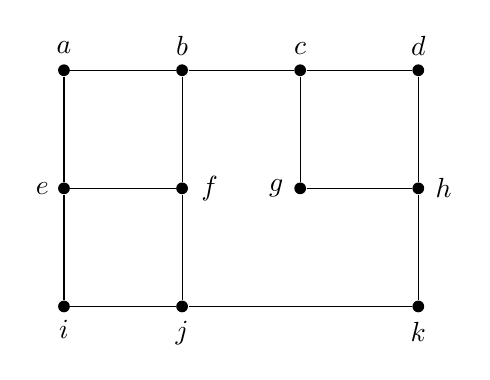
\begin{tikzpicture}[every node/.style={circle,fill,minimum size=1px,inner sep=1.5pt}]
    \node[label=90:$a$] (a) at (0,0) {};
    \node[label=90:$b$] (b) at (1.5,0) {};
    \node[label=90:$c$] (c) at (3,0) {};
    \node[label=90:$d$] (d) at (4.5,0) {};
    \node[label=180:$e$] (e) at (0,-1.5) {};
    \node[label=0:$f$] (f) at (1.5,-1.5) {};
    \node[label=180:$g$] (g) at (3,-1.5) {};
    \node[label=0:$h$] (h) at (4.5,-1.5) {};
    \node[label=270:$i$] (i) at (0,-3) {};
    \node[label=270:$j$] (j) at (1.5,-3) {};
    \node[label=270:$k$] (k) at (4.5,-3) {};
    
    \draw (a) -- (b);
    \draw (a) -- (e);
    \draw (b) -- (c);
    \draw (b) -- (f);
    \draw (c) -- (d);
    \draw (c) -- (g);
    \draw (d) -- (h);
    \draw (e) -- (f);
    \draw (e) -- (i);
    \draw (f) -- (j);
    \draw (g) -- (h);
    \draw (h) -- (k);
    \draw (i) -- (j);
    \draw (j) -- (k);
\end{tikzpicture}
\end{center}

The graph G contains 11 vertices. Let C be the set containing the three vertices. Then, every vertex in G is either in C or adjacent to a vertex in C. Since the maximum possible degree in G is 3, no vertex can cover more than 3 vertices. Also, since the vertices in C account for their self, 8 remaining vertices are left to be covered, implying that potential solutions take the form of
\begin{center}
    &(1) 3 vertices of degree 3 with 1 overlap \\
    &or \\
    &(2) 2 vertices of degree 3 and 1 vertex of degree 2 with \underline{no} overlap
\end{center}

\vspace{1em}

\underline{Choose}: a

\begin{center}
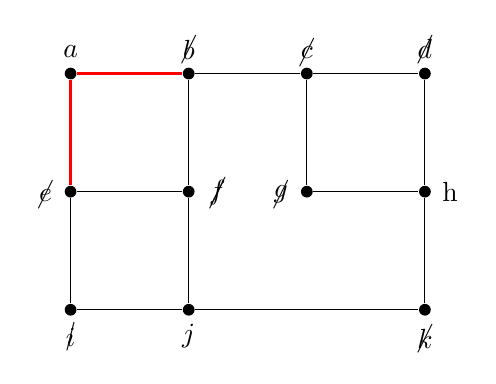
\begin{tikzpicture}[every node/.style={circle,fill,minimum size=1px,inner sep=1.5pt}]
    \node[label=90:${a}$] (a) at (0,0) {};
    \node[label=90:\cancel{$b$}] (b) at (1.5,0) {};
    \node[label=90:\cancel{${c}$}] (c) at (3,0) {};
    \node[label=90:\cancel{$d$}] (d) at (4.5,0) {};
    \node[label=180:\cancel{$e$}] (e) at (0,-1.5) {};
    \node[label=0:\cancel{${f}$}] (f) at (1.5,-1.5) {};
    \node[label=180:\cancel{$g$}] (g) at (3,-1.5) {};
    \node[label=0:h] (h) at (4.5,-1.5) {};
    \node[label=270:\cancel{$i$}] (i) at (0,-3) {};
    \node[label=270:$j$] (j) at (1.5,-3) {};
    \node[label=270:\cancel{$k$}] (k) at (4.5,-3) {};
    
    \draw (a) -- (b);
    \draw (a) -- (e);
    \draw (b) -- (c);
    \draw (b) -- (f);
    \draw (c) -- (d);
    \draw (c) -- (g);
    \draw (d) -- (h);
    \draw (e) -- (f);
    \draw (e) -- (i);
    \draw (f) -- (j);
    \draw (g) -- (h);
    \draw (h) -- (k);
    \draw (i) -- (j);
    \draw (j) -- (k);
    
    \draw[red,thick] (a) -- (b);
    \draw[red,thick] (a) -- (e);
\end{tikzpicture}
\\
- Eliminates e, c, b, f (By (2): no overlap can happen with a since it's degree 2) \\ 
- Eliminates i, g, k, d (By (2): can only have 1 vertex of degree 2) \\
$\Rightarrow$ \ not possible, c can not be covered \\
$\Rightarrow$ \ no solution exists with $|C| = 3$ containing a. 
\end{center}

\vspace{1em}

\underline{Backtrack} from a
\begin{center}

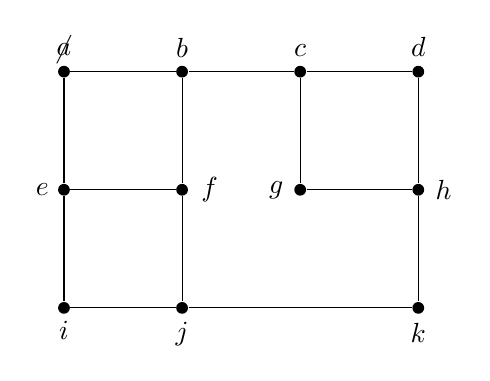
\begin{tikzpicture}[every node/.style={circle,fill,minimum size=1px,inner sep=1.5pt}]
    \node[label=90:\cancel{$a$}] (a) at (0,0) {};
    \node[label=90:$b$] (b) at (1.5,0) {};
    \node[label=90:$c$] (c) at (3,0) {};
    \node[label=90:$d$] (d) at (4.5,0) {};
    \node[label=180:$e$] (e) at (0,-1.5) {};
    \node[label=0:$f$] (f) at (1.5,-1.5) {};
    \node[label=180:$g$] (g) at (3,-1.5) {};
    \node[label=0:$h$] (h) at (4.5,-1.5) {};
    \node[label=270:$i$] (i) at (0,-3) {};
    \node[label=270:$j$] (j) at (1.5,-3) {};
    \node[label=270:$k$] (k) at (4.5,-3) {};
    
    \draw (a) -- (b);
    \draw (a) -- (e);
    \draw (b) -- (c);
    \draw (b) -- (f);
    \draw (c) -- (d);
    \draw (c) -- (g);
    \draw (d) -- (h);
    \draw (e) -- (f);
    \draw (e) -- (i);
    \draw (f) -- (j);
    \draw (g) -- (h);
    \draw (h) -- (k);
    \draw (i) -- (j);
    \draw (j) -- (k);
\end{tikzpicture}
\end{center}

\vspace{1em}

\underline{Choose}: b
\begin{center}
    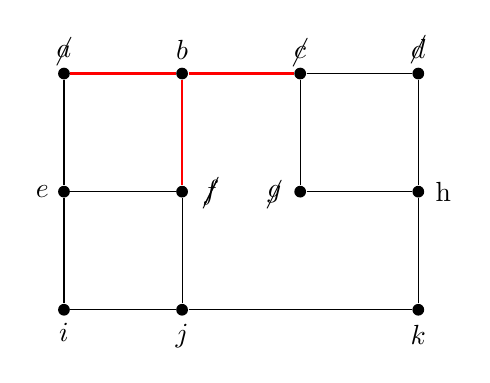
\begin{tikzpicture}[every node/.style={circle,fill,minimum size=1px,inner sep=1.5pt}]
    \node[label=90:$\cancel{a}$] (a) at (0,0) {};
    \node[label=90:$b$] (b) at (1.5,0) {};
    \node[label=90:$\cancel{c}$] (c) at (3,0) {};
    \node[label=90:$\cancel{d}$] (d) at (4.5,0) {};
    \node[label=180:$e$] (e) at (0,-1.5) {};
    \node[label=0:$\cancel{f}$] (f) at (1.5,-1.5) {};
    \node[label=180:$\cancel{g}$] (g) at (3,-1.5) {};
    \node[label=0:h] (h) at (4.5,-1.5) {};
    \node[label=270:$i$] (i) at (0,-3) {};
    \node[label=270:$j$] (j) at (1.5,-3) {};
    \node[label=270:$k$] (k) at (4.5,-3) {};
    
    \draw (a) -- (b);
    \draw (a) -- (e);
    \draw (b) -- (c);
    \draw (b) -- (f);
    \draw (c) -- (d);
    \draw (c) -- (g);
    \draw (d) -- (h);
    \draw (e) -- (f);
    \draw (e) -- (i);
    \draw (f) -- (j);
    \draw (g) -- (h);
    \draw (h) -- (k);
    \draw (i) -- (j);
    \draw (j) -- (k);
    
    \draw[red,thick] (a) -- (b);
    \draw[red,thick] (b) -- (f);
    \draw[red,thick] (b) -- (c);
\end{tikzpicture} \\
- Eliminates d and g (By (1): d and g are degree 2 but overlap with b)
\end{center}

\vspace{1em}

\underline{Choose}: h (covers d, g)
\begin{center}
    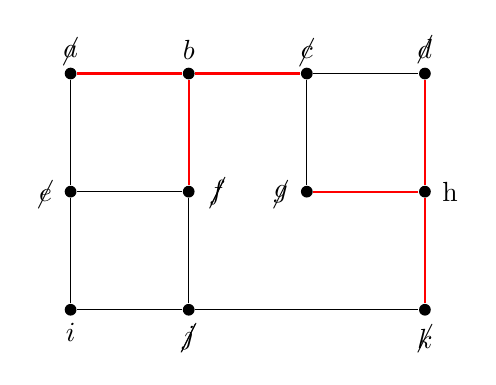
\begin{tikzpicture}[every node/.style={circle,fill,minimum size=1px,inner sep=1.5pt}]
    \node[label=90:$\cancel{a}$] (a) at (0,0) {};
    \node[label=90:$b$] (b) at (1.5,0) {};
    \node[label=90:$\cancel{c}$] (c) at (3,0) {};
    \node[label=90:$\cancel{d}$] (d) at (4.5,0) {};
    \node[label=180:$\cancel{e}$] (e) at (0,-1.5) {};
    \node[label=0:$\cancel{f}$] (f) at (1.5,-1.5) {};
    \node[label=180:$\cancel{g}$] (g) at (3,-1.5) {};
    \node[label=0:h] (h) at (4.5,-1.5) {};
    \node[label=270:$i$] (i) at (0,-3) {};
    \node[label=270:$\cancel{j}$] (j) at (1.5,-3) {};
    \node[label=270:\cancel{$k$}] (k) at (4.5,-3) {};
    
    \draw (a) -- (b);
    \draw (a) -- (e);
    \draw (b) -- (c);
    \draw (b) -- (f);
    \draw (c) -- (d);
    \draw (c) -- (g);
    \draw (d) -- (h);
    \draw (e) -- (f);
    \draw (e) -- (i);
    \draw (f) -- (j);
    \draw (g) -- (h);
    \draw (h) -- (k);
    \draw (i) -- (j);
    \draw (j) -- (k);
    
    \draw[red,thick] (a) -- (b);
    \draw[red,thick] (b) -- (f);
    \draw[red,thick] (b) -- (c);
    \draw[red,thick] (h) -- (d);
    \draw[red,thick] (h) -- (g);
    \draw[red,thick] (h) -- (k);
\end{tikzpicture} \\
\end{center}

\vspace{1em}
\\ 
\underline{Force}: i (covers e, j)
\begin{center}
    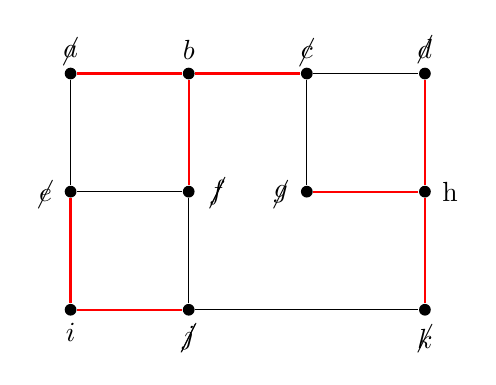
\begin{tikzpicture}[every node/.style={circle,fill,minimum size=1px,inner sep=1.5pt}]
    \node[label=90:$\cancel{a}$] (a) at (0,0) {};
    \node[label=90:$b$] (b) at (1.5,0) {};
    \node[label=90:$\cancel{c}$] (c) at (3,0) {};
    \node[label=90:$\cancel{d}$] (d) at (4.5,0) {};
    \node[label=180:$\cancel{e}$] (e) at (0,-1.5) {};
    \node[label=0:$\cancel{f}$] (f) at (1.5,-1.5) {};
    \node[label=180:$\cancel{g}$] (g) at (3,-1.5) {};
    \node[label=0:h] (h) at (4.5,-1.5) {};
    \node[label=270:$i$] (i) at (0,-3) {};
    \node[label=270:$\cancel{j}$] (j) at (1.5,-3) {};
    \node[label=270:\cancel{$k$}] (k) at (4.5,-3) {};
    
    \draw (a) -- (b);
    \draw (a) -- (e);
    \draw (b) -- (c);
    \draw (b) -- (f);
    \draw (c) -- (d);
    \draw (c) -- (g);
    \draw (d) -- (h);
    \draw (e) -- (f);
    \draw (e) -- (i);
    \draw (f) -- (j);
    \draw (g) -- (h);
    \draw (h) -- (k);
    \draw (i) -- (j);
    \draw (j) -- (k);
    
    \draw[red,thick] (a) -- (b);
    \draw[red,thick] (b) -- (f);
    \draw[red,thick] (b) -- (c);
    \draw[red,thick] (h) -- (d);
    \draw[red,thick] (h) -- (g);
    \draw[red,thick] (h) -- (k);
    \draw[red, thick] (i) -- (e);
    \draw[red, thick] (i) -- (j);
\end{tikzpicture} \\
\Rightarrow \ (1) \ \boxed{\{b, h, i\}}
\end{center}

\vspace{1em} \\

\underline{Backtrack} from h
\begin{center}
    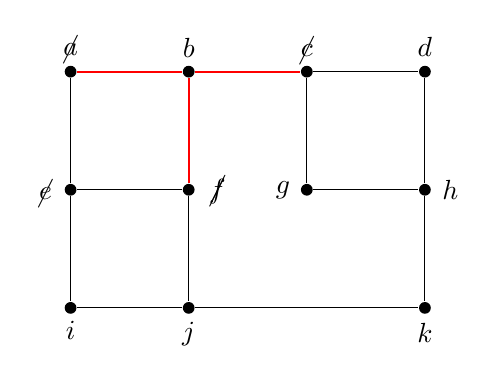
\begin{tikzpicture}[every node/.style={circle,fill,minimum size=1px,inner sep=1.5pt}]
    \node[label=90:$\cancel{a}$] (a) at (0,0) {};
    \node[label=90:$b$] (b) at (1.5,0) {};
    \node[label=90:$\cancel{c}$] (c) at (3,0) {};
    \node[label=90:$d$] (d) at (4.5,0) {};
    \node[label=180:$\cancel{e}$] (e) at (0,-1.5) {};
    \node[label=0:$\cancel{f}$] (f) at (1.5,-1.5) {};
    \node[label=180:$g$] (g) at (3,-1.5) {};
    \node[label=0:$h$] (h) at (4.5,-1.5) {};
    \node[label=270:$i$] (i) at (0,-3) {};
    \node[label=270:$j$] (j) at (1.5,-3) {};
    \node[label=270:$k$] (k) at (4.5,-3) {};
    
    \draw (a) -- (b);
    \draw (a) -- (e);
    \draw (b) -- (c);
    \draw (b) -- (f);
    \draw (c) -- (d);
    \draw (c) -- (g);
    \draw (d) -- (h);
    \draw (e) -- (f);
    \draw (e) -- (i);
    \draw (f) -- (j);
    \draw (g) -- (h);
    \draw (h) -- (k);
    \draw (i) -- (j);
    \draw (j) -- (k);
    
    \draw[red,thick] (a) -- (b);
    \draw[red,thick] (b) -- (f);
    \draw[red,thick] (b) -- (c);
\end{tikzpicture} \\
- Eliminates e (By (1), e has 2 overlaps with b)
\end{center} 

\vspace{1em}

\underline{Force}: c

\begin{center}
    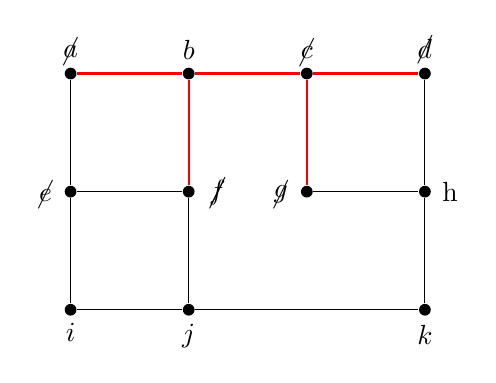
\begin{tikzpicture}[every node/.style={circle,fill,minimum size=1px,inner sep=1.5pt}]
    \node[label=90:$\cancel{a}$] (a) at (0,0) {};
    \node[label=90:$b$] (b) at (1.5,0) {};
    \node[label=90:$\cancel{c}$] (c) at (3,0) {};
    \node[label=90:$\cancel{d}$] (d) at (4.5,0) {};
    \node[label=180:$\cancel{e}$] (e) at (0,-1.5) {};
    \node[label=0:$\cancel{f}$] (f) at (1.5,-1.5) {};
    \node[label=180:$\cancel{g}$] (g) at (3,-1.5) {};
    \node[label=0:h] (h) at (4.5,-1.5) {};
    \node[label=270:$i$] (i) at (0,-3) {};
    \node[label=270:$j$] (j) at (1.5,-3) {};
    \node[label=270:$k$] (k) at (4.5,-3) {};
    
    \draw (a) -- (b);
    \draw (a) -- (e);
    \draw (b) -- (c);
    \draw (b) -- (f);
    \draw (c) -- (d);
    \draw (c) -- (g);
    \draw (d) -- (h);
    \draw (e) -- (f);
    \draw (e) -- (i);
    \draw (f) -- (j);
    \draw (g) -- (h);
    \draw (h) -- (k);
    \draw (i) -- (j);
    \draw (j) -- (k);
    
    \draw[red,thick] (a) -- (b);
    \draw[red,thick] (b) -- (f);
    \draw[red,thick] (b) -- (c);
    \draw[red, thick] (c) -- (d);
    \draw[red, thick] (c) -- (g);
\end{tikzpicture} \\
$\Rightarrow$ \ Not possible by (1), either e, j, or h will cause an extra overlap either with b or c. \\ 
$\Rightarrow$ \ No solution exists with $|C| = 3$ containing b, c
\end{center}

\vspace{1em}

\underline{Force}: e (covers a)

\begin{center}
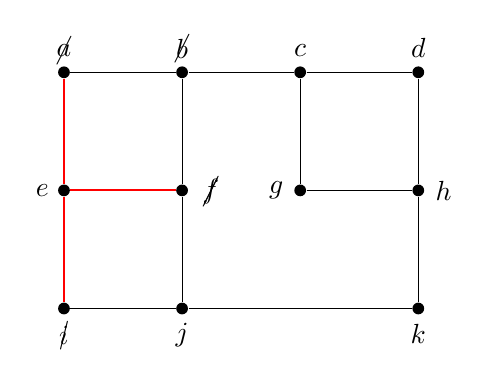
\begin{tikzpicture}[every node/.style={circle,fill,minimum size=1px,inner sep=1.5pt}]
    \node[label=90:$\cancel{a}$] (a) at (0,0) {};
    \node[label=90:$\cancel{b}$] (b) at (1.5,0) {};
    \node[label=90:${c}$] (c) at (3,0) {};
    \node[label=90:$d$] (d) at (4.5,0) {};
    \node[label=180:$e$] (e) at (0,-1.5) {};
    \node[label=0:$\cancel{f}$] (f) at (1.5,-1.5) {};
    \node[label=180:$g$] (g) at (3,-1.5) {};
    \node[label=0:$h$] (h) at (4.5,-1.5) {};
    \node[label=270:$\cancel{i}$] (i) at (0,-3) {};
    \node[label=270:$j$] (j) at (1.5,-3) {};
    \node[label=270:$k$] (k) at (4.5,-3) {};
    
    \draw (a) -- (b);
    \draw (a) -- (e);
    \draw (b) -- (c);
    \draw (b) -- (f);
    \draw (c) -- (d);
    \draw (c) -- (g);
    \draw (d) -- (h);
    \draw (e) -- (f);
    \draw (e) -- (i);
    \draw (f) -- (j);
    \draw (g) -- (h);
    \draw (h) -- (k);
    \draw (i) -- (j);
    \draw (j) -- (k);
    
    \draw[red,thick] (a) -- (e);
    \draw[red,thick] (e) -- (f);
    \draw[red,thick] (e) -- (i);
\end{tikzpicture} \\
- Eliminates b (by (1), b would cause 2 overlaps with e)
- Eliminates i (by (2), i overlaps with e)
\end{center}

\vspace{1em}
\\
\underline{Choose}: c
\begin{center}
    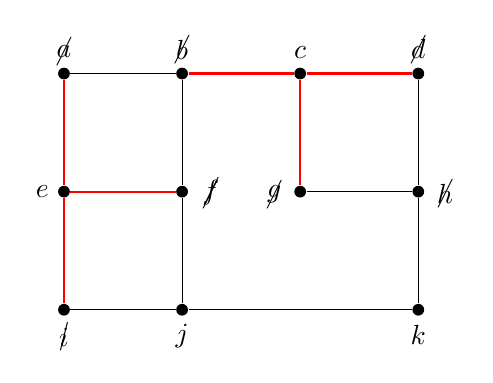
\begin{tikzpicture}[every node/.style={circle,fill,minimum size=1px,inner sep=1.5pt}]
    \node[label=90:$\cancel{a}$] (a) at (0,0) {};
    \node[label=90:$\cancel{b}$] (b) at (1.5,0) {};
    \node[label=90:${c}$] (c) at (3,0) {};
    \node[label=90:$\cancel{d}$] (d) at (4.5,0) {};
    \node[label=180:$e$] (e) at (0,-1.5) {};
    \node[label=0:$\cancel{f}$] (f) at (1.5,-1.5) {};
    \node[label=180:$\cancel{g}$] (g) at (3,-1.5) {};
    \node[label=0:$\cancel{h}$] (h) at (4.5,-1.5) {};
    \node[label=270:$\cancel{i}$] (i) at (0,-3) {};
    \node[label=270:$j$] (j) at (1.5,-3) {};
    \node[label=270:$k$] (k) at (4.5,-3) {};
    
    \draw (a) -- (b);
    \draw (a) -- (e);
    \draw (b) -- (c);
    \draw (b) -- (f);
    \draw (c) -- (d);
    \draw (c) -- (g);
    \draw (d) -- (h);
    \draw (e) -- (f);
    \draw (e) -- (i);
    \draw (f) -- (j);
    \draw (g) -- (h);
    \draw (h) -- (k);
    \draw (i) -- (j);
    \draw (j) -- (k);
    
     \draw[red,thick] (a) -- (e);
    \draw[red,thick] (e) -- (f);
    \draw[red,thick] (e) -- (i);
    \draw[red, thick] (c) -- (g);
    \draw[red, thick] (c) -- (b);
    \draw[red, thick] (c) -- (d);
\end{tikzpicture} \\
- Eliminates h (by (1), h has 2 overlaps with c)
\end{center}

\vspace{1em} \\
\underline{Force}: k (covers j and h)
\begin{center}
    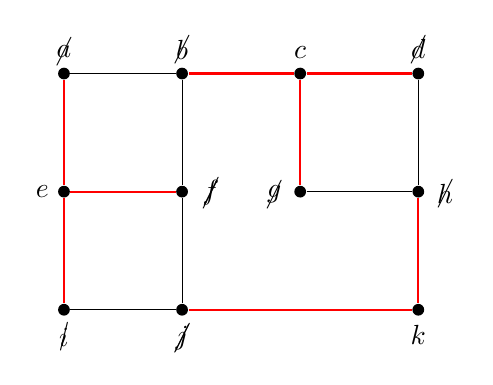
\begin{tikzpicture}[every node/.style={circle,fill,minimum size=1px,inner sep=1.5pt}]
    \node[label=90:$\cancel{a}$] (a) at (0,0) {};
    \node[label=90:$\cancel{b}$] (b) at (1.5,0) {};
    \node[label=90:${c}$] (c) at (3,0) {};
    \node[label=90:$\cancel{d}$] (d) at (4.5,0) {};
    \node[label=180:$e$] (e) at (0,-1.5) {};
    \node[label=0:$\cancel{f}$] (f) at (1.5,-1.5) {};
    \node[label=180:$\cancel{g}$] (g) at (3,-1.5) {};
    \node[label=0:$\cancel{h}$] (h) at (4.5,-1.5) {};
    \node[label=270:$\cancel{i}$] (i) at (0,-3) {};
    \node[label=270:$\cancel{j}$] (j) at (1.5,-3) {};
    \node[label=270:$k$] (k) at (4.5,-3) {};
    
    \draw (a) -- (b);
    \draw (a) -- (e);
    \draw (b) -- (c);
    \draw (b) -- (f);
    \draw (c) -- (d);
    \draw (c) -- (g);
    \draw (d) -- (h);
    \draw (e) -- (f);
    \draw (e) -- (i);
    \draw (f) -- (j);
    \draw (g) -- (h);
    \draw (h) -- (k);
    \draw (i) -- (j);
    \draw (j) -- (k);
    
    \draw[red,thick] (a) -- (e);
    \draw[red,thick] (e) -- (f);
    \draw[red,thick] (e) -- (i);
    \draw[red, thick] (c) -- (g);
    \draw[red, thick] (c) -- (b);
    \draw[red, thick] (c) -- (d);
    \draw[red, thick] (k) -- (j);
    \draw[red, thick] (k) -- (h);
\end{tikzpicture}
\end{center}

\begin{center}
    \Rightarrow \ (2) \  \boxed{$\{e, c, k\}$}
\end{center}

\vspace{1em}
\underline{Backtrack} from c

\begin{center}
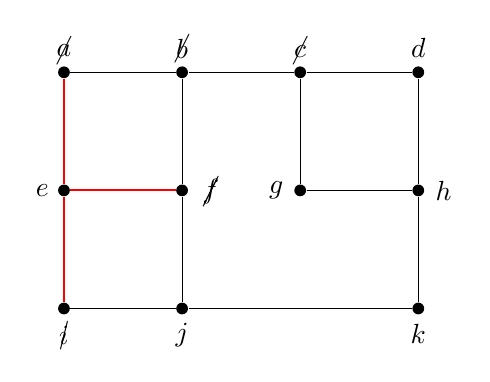
\begin{tikzpicture}[every node/.style={circle,fill,minimum size=1px,inner sep=1.5pt}]
    \node[label=90:$\cancel{a}$] (a) at (0,0) {};
    \node[label=90:$\cancel{b}$] (b) at (1.5,0) {};
    \node[label=90:$\cancel{c}$] (c) at (3,0) {};
    \node[label=90:$d$] (d) at (4.5,0) {};
    \node[label=180:$e$] (e) at (0,-1.5) {};
    \node[label=0:$\cancel{f}$] (f) at (1.5,-1.5) {};
    \node[label=180:$g$] (g) at (3,-1.5) {};
    \node[label=0:$h$] (h) at (4.5,-1.5) {};
    \node[label=270:$\cancel{i}$] (i) at (0,-3) {};
    \node[label=270:$j$] (j) at (1.5,-3) {};
    \node[label=270:$k$] (k) at (4.5,-3) {};
    
    \draw (a) -- (b);
    \draw (a) -- (e);
    \draw (b) -- (c);
    \draw (b) -- (f);
    \draw (c) -- (d);
    \draw (c) -- (g);
    \draw (d) -- (h);
    \draw (e) -- (f);
    \draw (e) -- (i);
    \draw (f) -- (j);
    \draw (g) -- (h);
    \draw (h) -- (k);
    \draw (i) -- (j);
    \draw (j) -- (k);
    
    \draw[red,thick] (a) -- (e);
    \draw[red,thick] (e) -- (f);
    \draw[red,thick] (e) -- (i);
\end{tikzpicture} \\
\end{center}


\vspace{1em}
\\ 
\underline{Force}: h
\begin{center}
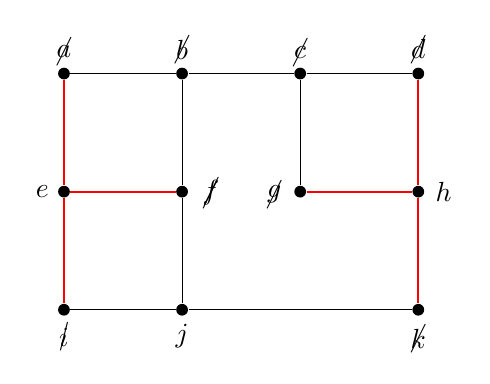
\begin{tikzpicture}[every node/.style={circle,fill,minimum size=1px,inner sep=1.5pt}]
    \node[label=90:$\cancel{a}$] (a) at (0,0) {};
    \node[label=90:$\cancel{b}$] (b) at (1.5,0) {};
    \node[label=90:$\cancel{c}$] (c) at (3,0) {};
    \node[label=90:$\cancel{d}$] (d) at (4.5,0) {};
    \node[label=180:$e$] (e) at (0,-1.5) {};
    \node[label=0:$\cancel{f}$] (f) at (1.5,-1.5) {};
    \node[label=180:$\cancel{g}$] (g) at (3,-1.5) {};
    \node[label=0:$h$] (h) at (4.5,-1.5) {};
    \node[label=270:$\cancel{i}$] (i) at (0,-3) {};
    \node[label=270:$j$] (j) at (1.5,-3) {};
    \node[label=270:$\cancel{k}$] (k) at (4.5,-3) {};
    
    \draw (a) -- (b);
    \draw (a) -- (e);
    \draw (b) -- (c);
    \draw (b) -- (f);
    \draw (c) -- (d);
    \draw (c) -- (g);
    \draw (d) -- (h);
    \draw (e) -- (f);
    \draw (e) -- (i);
    \draw (f) -- (j);
    \draw (g) -- (h);
    \draw (h) -- (k);
    \draw (i) -- (j);
    \draw (j) -- (k);
    
    \draw[red,thick] (a) -- (e);
    \draw[red,thick] (e) -- (f);
    \draw[red,thick] (e) -- (i);
    \draw[red,thick] (h) -- (g);
    \draw[red,thick] (h) -- (d);
    \draw[red,thick] (h) -- (k);
\end{tikzpicture} \\
$\Rightarrow$ \ Not possible by (1), j creates 2 overlaps with e. \\
$\Rightarrow$ \ No solution exists with $|C| = 3$ containing e, j, and k.
\end{center}

 
 
\begin{center}
    All choices have been exausted and $\therefore$ all solutions have been found.
\end{center}

\end{document}